\section{Randomized Computation - 随机计算}
To demonstrate how randomized computation speeds up compared to deterministic computation, we can consider the following examples.

\subsection{A Simple Example}
Consider that you are given a string of $n$ bits, which are promised to be either all $0$s or exactly half of the bits are $1$s, find an algorithm to decide which case you are in. \\
Deterministically, the time complexity is $\Theta(n)$ as you need to try at least $\frac{n}{2}$ times, and at most $n$ times. \\
With a randomized algorithm, the time complexity is $\order{1}$, where we can obtain the correct answer with high probability. The description is simple,
\begin{quote}
    While we do not see a $1$, we select a bit randomly. If this bit is $1$, we say we are in the second case. Otherwise, we say we are in the first case, where the string is all $0$s.
\end{quote}
We run the above algorithm a constant number of times, say $c$. If the string is indeed all $0$s, the algorithm above is always correct. If the string is half $1$s, then the algorithm is correct with a probability of
\begin{align*}
    \Prob{\text{success}} &= \Prob{\text{seeing }1\text{ once among }c\text{ times}} \\
    &= 1 - \Prob{\text{seeing all }0} \\
    &= 1 - (\frac{1}{2})^c
\end{align*}
When the string is half $1$s, we can obtain the correct output with arbitarily high probability as we increase $c$. \\
This is a type of \impt{Monte Carlo} algorithm, where we have a fixed runtime, but can be wrong.

\subsection{NAND Tree Problem}
Consider an input of $n$ bits where $n := 2^h$. Say $h = 3$, we consider a balanced binary tree
\begin{center}
    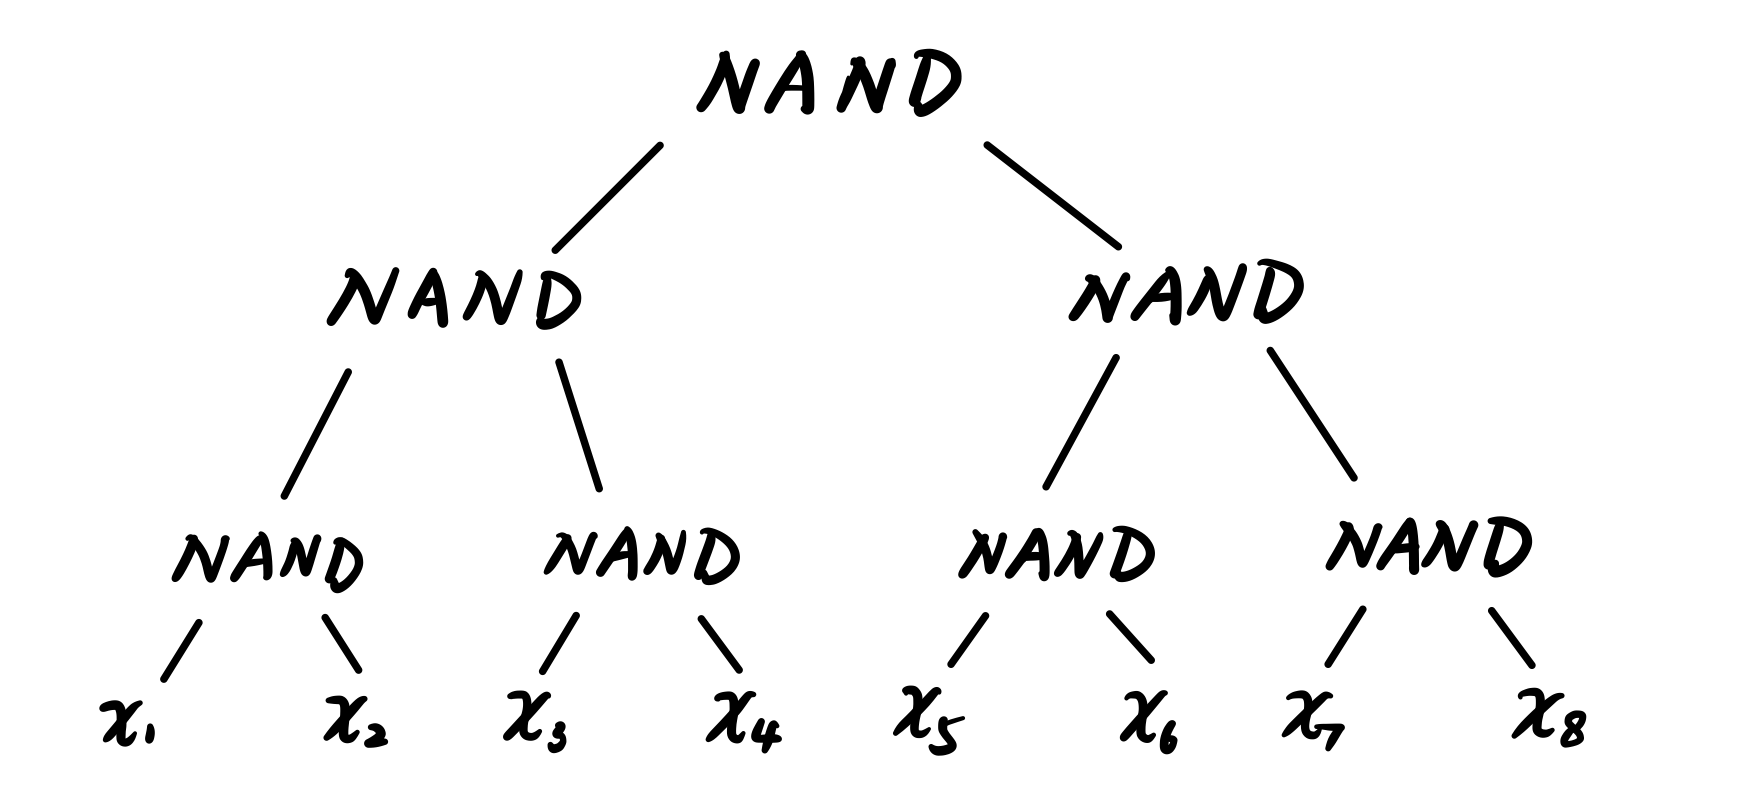
\includegraphics[scale = 0.15]{2/NAND tree.png}
\end{center}
We want to know the output of the root node. \\
Deterministically, the time complexity is $\Theta(n) = \Theta(2^h)$. \\
As for the randomized algorithm, we first consider a step of the algorithm, denoted as $\mathcal{A}_h$, where $h$ represents the height of the tree. This single step does one thing: starting from the root, examine left or right branch uniformly at random; if sees $0$, we output $1$; if sees $1$, we examine the other branch and the output NAND of both examinations. This is a recursive randomized algorithm. \\
We further denote $\alpha_b(h)$ to be the expected complexity of $\mathcal{A}_h$ if input $\mathbf{x}$ maps to $b$. \\
Then, we have:
\begin{align*}
    \alpha_0(h) &\le 2\alpha_1(h - 1) \\
    \alpha_1(h) &\le \max \begin{cases}
        \alpha_0(h - 1) \\
        \alpha_0(h - 1) + \frac{1}{2} \alpha_1(h - 1) \\
        \alpha_0(h - 1) + \frac{1}{2} \alpha_1(h - 1)
    \end{cases} \\
    &\le 2\alpha_1(h - 2) + \frac{1}{2}\alpha_1(h - 1)
\end{align*}
These inequalities stand from the NAND operations where:
\begin{align*}
    0 \text{ NAND } 0 &= 1 \\ 
    0 \text{ NAND } 1 &= 1 \\ 
    1 \text{ NAND } 0 &= 1 \\
    1 \text{ NAND } 1 &= 0
\end{align*}
And this algorithm solves to have a complexity of $\sim \order{1.686^h}$. \\
This is a type of \impt{Las Vegas} algorithm, where we have unfixed runtime, but the output is always correct.

\subsection{Randomized vs. Deterministic Algorithms}
A randomized algorithm can be thought of as choosing from some distribution of deterministic algorithms. If we require the randomized algorithms to have both fixed runtime and the output to be always correct, then there is no advantage from randomization. \\
We cover randomized algorithms because many quantum algorithms employ randomness and we want to show that quantum algorithms can be strictly faster than randomized algorithms (otherwise, speedup from randomization would be enough).

\subsection{Randomized State - 随机态}
\begin{definition}
    A \uimpt{randomized state} on $n$ bits is described by a column vector of length $2^n$
    $$\vec{p} = (p_{00 \dots 0}, p_{00 \dots 1}, \dots, p_{11 \dots 1})^\top$$
    such that it satisfies two conditions:
    \begin{quote}
        1. Normalization: $\Sumi{\mathbf{x}} p_{\mathbf{x}} = 1$. \\
        2. Non-negativity: $\forall p_{\mathbf{x}}, p_{\mathbf{x}} \ge 0$
    \end{quote}
\end{definition}
If exactly one of $p_{\mathbf{x}} \ne 0$, we refer to $\vec{p}$ as a \impt{deterministic state}, corresponding to bitstring $\mathbf{x}$. \\
Note that \impt{doing operations on randomized states in different orders can change the outcome}. We can also consider doing randomized operations on randomized states as well.

\subsection{Randomized Operation - 随机过程}
\begin{definition}
    A \uimpt{randomized operation} (a.k.a stochastic operation/matrix) acting on $n$ bits is described by a $2^n \times 2^n$ matrix $A$, such that:
    \begin{quote}
        1. All entries of $A$ are non-negative, \\
        2. Sum of every column is $1$.
    \end{quote}
\end{definition}
This implies that every column is a randomized state. If every column is a deterministic state, then we say $A$ is a \impt{deterministic operation}. \\
For example, a coin flip on $1$ bit can be characterized as
$$A = \begin{pmatrix}
    \frac{1}{2} & \frac{1}{2} \\
    \frac{1}{2} & \frac{1}{2}
\end{pmatrix}$$
\begin{lemma}
    A randomized operation that acts on a randomized state will yield a randomized state.
\end{lemma}

\subsection{Other Important Concepts}
The \impt{tensor product} of randomized states can be regarded as the following. Consider a $2$-bit state, where the first bit is determined by a fair coin, while the second bit is set to $0$. If we wish to describe the final state, we have:
$$\begin{pmatrix}
    \frac{1}{2} \\ \frac{1}{2}
\end{pmatrix} \otimes \begin{pmatrix}
    1 \\ 0
\end{pmatrix} = \begin{pmatrix}
    \frac{1}{2} \begin{pmatrix}
        1 \\ 0
    \end{pmatrix} \\ \frac{1}{2} \begin{pmatrix}
        1 \\ 0
    \end{pmatrix}
\end{pmatrix} = \begin{pmatrix}
    \frac{1}{2} \\ 0 \\ \frac{1}{2} \\ 0
\end{pmatrix}$$
Similarly, an example of the tensor product of randomized operations is the following:
$$\text{NOT} \otimes \id$$
A \impt{randomized circuit} is a circuit consisting of randomized operations. \\
\impt{Measuring a randomized state} on $n$ bits, $\vec{p}$, is a procedure that outputs $\mathbf{x} \in \{0, 1\}^n$ with probability $p_{\mathbf{x}}$. \\
The process of randomized computation consists of input bits and \impt{ancillas} that goes through a randomized circuit and obtain an output through a measurement. \\
For randomized computation, the Toffoli gate and the CNOT operation is universal -- any randomized computation can be decomposed into a sequence of these 2 operations to arbitrary precision.

\newpage